% Created 2019-04-05 vie 12:41
% Intended LaTeX compiler: pdflatex
\documentclass[11pt]{article}
\usepackage[utf8]{inputenc}
\usepackage[T1]{fontenc}
\usepackage{graphicx}
\usepackage{grffile}
\usepackage{longtable}
\usepackage{wrapfig}
\usepackage{rotating}
\usepackage[normalem]{ulem}
\usepackage{amsmath}
\usepackage{textcomp}
\usepackage{amssymb}
\usepackage{capt-of}
\usepackage{hyperref}
\author{Marco Sua}
\date{\today}
\title{Programación Lineal}
\hypersetup{
 pdfauthor={Marco Sua},
 pdftitle={Programación Lineal},
 pdfkeywords={},
 pdfsubject={},
 pdfcreator={Emacs 25.2.2 (Org mode 9.2.1)}, 
 pdflang={English}}
\begin{document}

\maketitle
\tableofcontents


\section{Teoría}
\label{sec:org3a9823e}
\subsection{Motivación}
\label{sec:orgadcef4f}

El objetivo de la programación lineal es maxizar funciones lineales
sobre dominios convexos, es decir, definidos sobre renglones dadas por
desigualdades.

\begin{center}
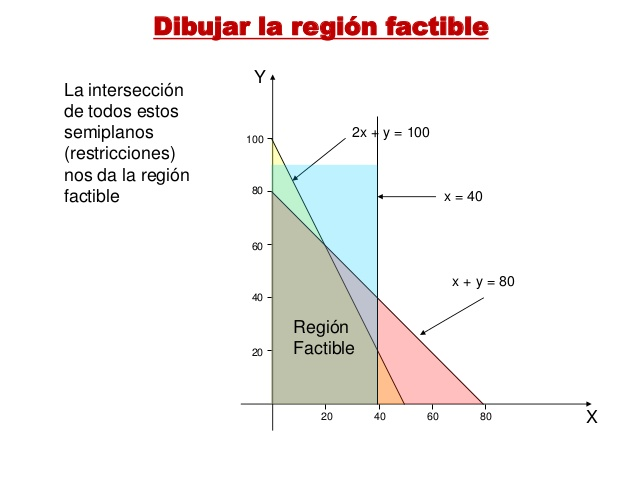
\includegraphics[width=.9\linewidth]{io-2da-programacion-lineal-32-638.jpg}
\end{center}
\subsection{Ejemplos}
\label{sec:orgcb02db4}

\begin{itemize}
\item El problema de la dieta.
\item Optimización de lugares en una excursión.
\item Escoger objetos óptimos para un campamento.
\item El problema del flujo máximo.
\end{itemize}

\subsection{Convexidad}
\label{sec:org9ae293c}

Un conjunto \(X\) es \textbf{convexo} sí para todos \(x,y\in X\) y \(t\in
   [0,1]\) se tiene que \(tx+(1-t)y\in X\).

\subsection{Método símplex}
\label{sec:orgca4fe21}

\section{Herramientas computacionales}
\label{sec:org397b552}
\subsection{Emacs}
\label{sec:orgf100d32}

\begin{center}
\begin{tabular}{ll}
C-x C-s & Salvar archivo\\
C-x C-f & Abrir archivo\\
M-q & Formatear el párrafo\\
C-x d & Editar directorio\\
C-g & Salir\\
C-x 2 & Divide horizontalmente\\
C-x 3 & Divide verticalmente\\
C-x 1 & Regresa a una sola pantalla\\
M-w & Copiar la región\\
C-w & Borrar la región\\
Shift y flechas & Seleccionar la región\\
C-y & Pegar la región\\
\end{tabular}
\end{center}

\subsection{Git}
\label{sec:org843cc13}
\begin{enumerate}
\item Git en la terminal
\label{sec:org8522778}
\item Github
\label{sec:orgc929355}
\end{enumerate}
\subsection{Python}
\label{sec:orgf7d7bf8}
\begin{enumerate}
\item El lenguaje de Python
\label{sec:org469c134}
\item Jupyter
\label{sec:org73dd99c}
\end{enumerate}
\subsection{Latex}
\label{sec:orged60103}
\end{document}